The Reporting module represents the core of the value that the users will
get out of the system. Reports are the means with which the users will
be able to see the results of the benchmarking of their programs.

\subsection{Scope}
The scope for the reporting module is shown in Figure \ref{fig:reportingScope}
\begin{figure}[H]
  \begin{center}
  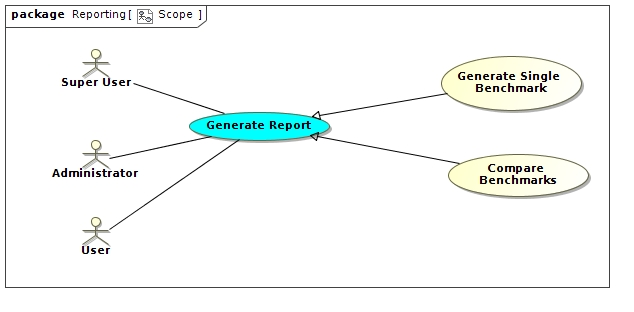
\includegraphics[scale=0.38]{../Diagrams and Charts/Reporting/Scope.jpg}
  \caption{Reporting Scope}
  \label{fig:reportingScope}
  \end{center}
\end{figure}


\subsection {Download Results}
The \textit{Download Results} use case is concerned with presenting the results
of a job to the user in a global interchange format, which was chosen
as CSV (Comma Seperated Value) representation.

\subsubsection{Service Contract}
The service contract for downloading results for a specified job is shown in 
Figure \ref{fig:downloadResultsServiceContract}
\begin{figure}[H]
  \begin{center}
  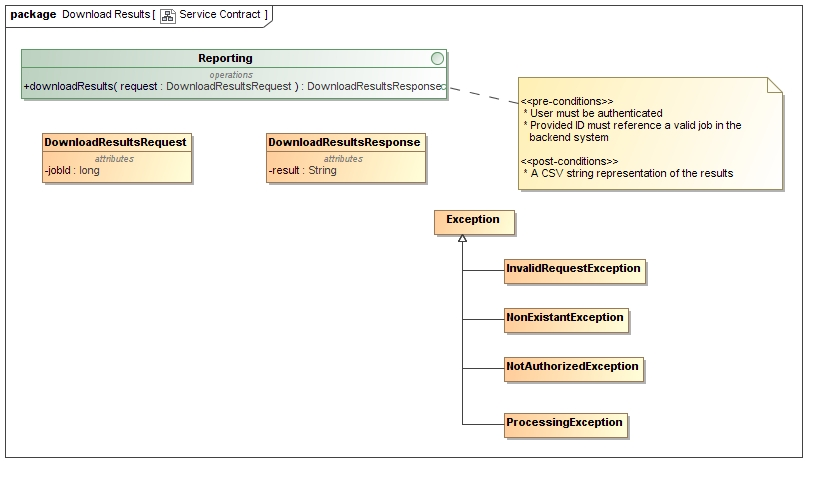
\includegraphics[scale=0.38]{../Diagrams and Charts/Reporting/Download Results Service Contract.jpg}
  \caption{Download Results Service Contract}
  \label{fig:downloadResultsServiceContract}
  \end{center}
\end{figure}


